% Created by tikzDevice version 0.12.3.1 on 2022-09-24 12:48:01
% !TEX encoding = UTF-8 Unicode
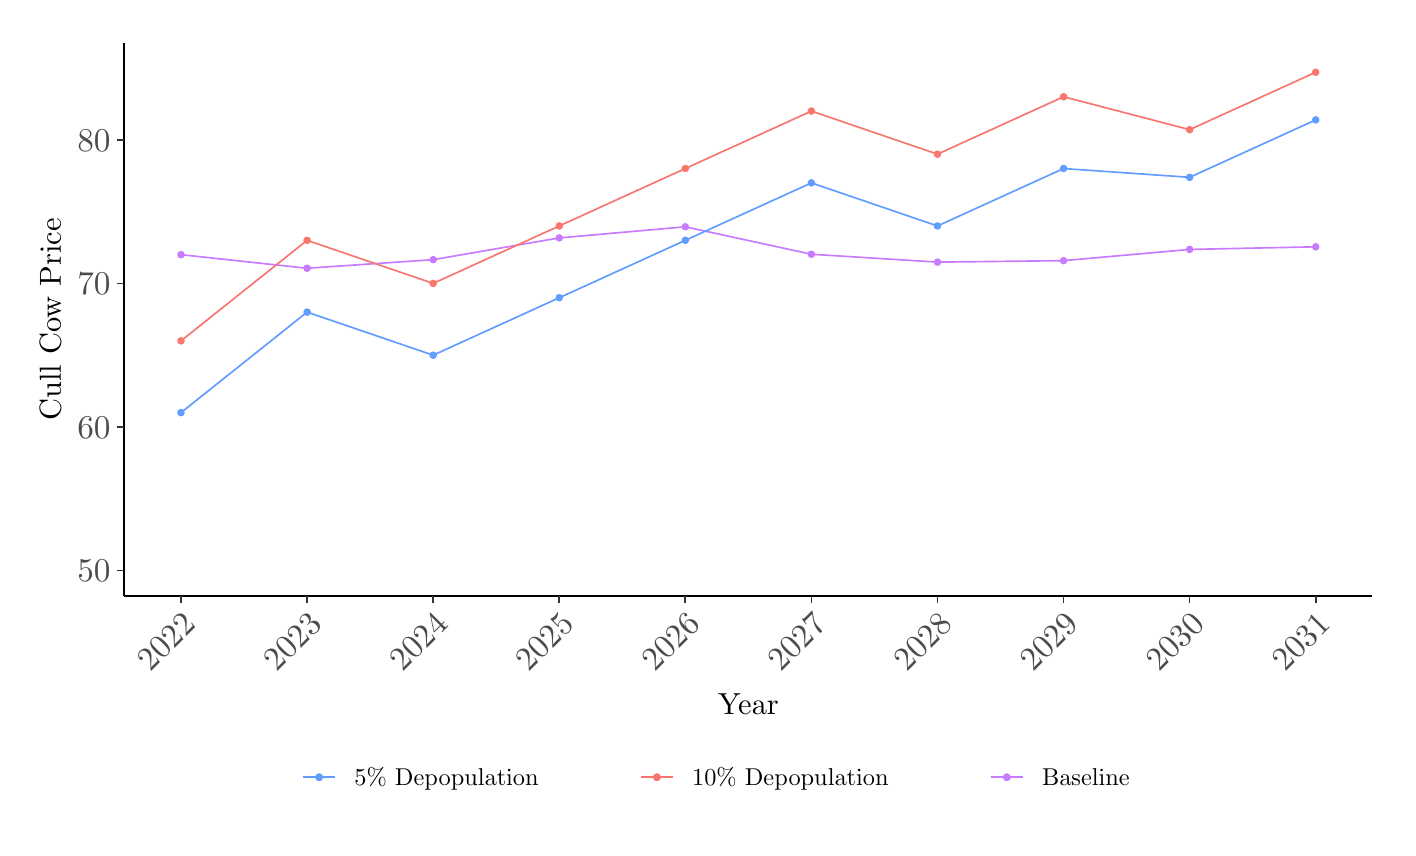
\begin{tikzpicture}[x=1pt,y=1pt]
\definecolor{fillColor}{RGB}{255,255,255}
\path[use as bounding box,fill=fillColor,fill opacity=0.00] (0,0) rectangle (491.44,289.08);
\begin{scope}
\path[clip] (  0.00,  0.00) rectangle (491.44,289.08);
\definecolor{drawColor}{RGB}{255,255,255}
\definecolor{fillColor}{RGB}{255,255,255}

\path[draw=drawColor,line width= 0.6pt,line join=round,line cap=round,fill=fillColor] (  0.00, -0.00) rectangle (491.44,289.08);
\end{scope}
\begin{scope}
\path[clip] ( 34.91, 83.83) rectangle (485.94,283.58);
\definecolor{fillColor}{RGB}{255,255,255}

\path[fill=fillColor] ( 34.91, 83.83) rectangle (485.94,283.58);
\definecolor{drawColor}{RGB}{199,124,255}

\path[draw=drawColor,line width= 0.6pt,line join=round] ( 55.41,207.05) --
	(100.97,202.14) --
	(146.53,205.25) --
	(192.09,213.11) --
	(237.64,217.12) --
	(283.20,207.21) --
	(328.76,204.36) --
	(374.32,204.89) --
	(419.88,208.94) --
	(465.43,209.89);
\definecolor{fillColor}{RGB}{199,124,255}

\path[draw=drawColor,line width= 0.4pt,line join=round,line cap=round,fill=fillColor] ( 55.41,207.05) circle (  1.16);

\path[draw=drawColor,line width= 0.4pt,line join=round,line cap=round,fill=fillColor] (100.97,202.14) circle (  1.16);

\path[draw=drawColor,line width= 0.4pt,line join=round,line cap=round,fill=fillColor] (146.53,205.25) circle (  1.16);

\path[draw=drawColor,line width= 0.4pt,line join=round,line cap=round,fill=fillColor] (192.09,213.11) circle (  1.16);

\path[draw=drawColor,line width= 0.4pt,line join=round,line cap=round,fill=fillColor] (237.64,217.12) circle (  1.16);

\path[draw=drawColor,line width= 0.4pt,line join=round,line cap=round,fill=fillColor] (283.20,207.21) circle (  1.16);

\path[draw=drawColor,line width= 0.4pt,line join=round,line cap=round,fill=fillColor] (328.76,204.36) circle (  1.16);

\path[draw=drawColor,line width= 0.4pt,line join=round,line cap=round,fill=fillColor] (374.32,204.89) circle (  1.16);

\path[draw=drawColor,line width= 0.4pt,line join=round,line cap=round,fill=fillColor] (419.88,208.94) circle (  1.16);

\path[draw=drawColor,line width= 0.4pt,line join=round,line cap=round,fill=fillColor] (465.43,209.89) circle (  1.16);
\definecolor{drawColor}{RGB}{97,156,255}

\path[draw=drawColor,line width= 0.6pt,line join=round] ( 55.41,149.98) --
	(100.97,186.30) --
	(146.53,170.73) --
	(192.09,191.49) --
	(237.64,212.24) --
	(283.20,232.99) --
	(328.76,217.43) --
	(374.32,238.18) --
	(419.88,235.00) --
	(465.43,255.75);
\definecolor{fillColor}{RGB}{97,156,255}

\path[draw=drawColor,line width= 0.4pt,line join=round,line cap=round,fill=fillColor] ( 55.41,149.98) circle (  1.16);

\path[draw=drawColor,line width= 0.4pt,line join=round,line cap=round,fill=fillColor] (100.97,186.30) circle (  1.16);

\path[draw=drawColor,line width= 0.4pt,line join=round,line cap=round,fill=fillColor] (146.53,170.73) circle (  1.16);

\path[draw=drawColor,line width= 0.4pt,line join=round,line cap=round,fill=fillColor] (192.09,191.49) circle (  1.16);

\path[draw=drawColor,line width= 0.4pt,line join=round,line cap=round,fill=fillColor] (237.64,212.24) circle (  1.16);

\path[draw=drawColor,line width= 0.4pt,line join=round,line cap=round,fill=fillColor] (283.20,232.99) circle (  1.16);

\path[draw=drawColor,line width= 0.4pt,line join=round,line cap=round,fill=fillColor] (328.76,217.43) circle (  1.16);

\path[draw=drawColor,line width= 0.4pt,line join=round,line cap=round,fill=fillColor] (374.32,238.18) circle (  1.16);

\path[draw=drawColor,line width= 0.4pt,line join=round,line cap=round,fill=fillColor] (419.88,235.00) circle (  1.16);

\path[draw=drawColor,line width= 0.4pt,line join=round,line cap=round,fill=fillColor] (465.43,255.75) circle (  1.16);
\definecolor{drawColor}{RGB}{248,118,109}

\path[draw=drawColor,line width= 0.6pt,line join=round] ( 55.41,175.92) --
	(100.97,212.24) --
	(146.53,196.67) --
	(192.09,217.43) --
	(237.64,238.18) --
	(283.20,258.94) --
	(328.76,243.37) --
	(374.32,264.12) --
	(419.88,252.22) --
	(465.43,272.97);
\definecolor{fillColor}{RGB}{248,118,109}

\path[draw=drawColor,line width= 0.4pt,line join=round,line cap=round,fill=fillColor] ( 55.41,175.92) circle (  1.16);

\path[draw=drawColor,line width= 0.4pt,line join=round,line cap=round,fill=fillColor] (100.97,212.24) circle (  1.16);

\path[draw=drawColor,line width= 0.4pt,line join=round,line cap=round,fill=fillColor] (146.53,196.67) circle (  1.16);

\path[draw=drawColor,line width= 0.4pt,line join=round,line cap=round,fill=fillColor] (192.09,217.43) circle (  1.16);

\path[draw=drawColor,line width= 0.4pt,line join=round,line cap=round,fill=fillColor] (237.64,238.18) circle (  1.16);

\path[draw=drawColor,line width= 0.4pt,line join=round,line cap=round,fill=fillColor] (283.20,258.94) circle (  1.16);

\path[draw=drawColor,line width= 0.4pt,line join=round,line cap=round,fill=fillColor] (328.76,243.37) circle (  1.16);

\path[draw=drawColor,line width= 0.4pt,line join=round,line cap=round,fill=fillColor] (374.32,264.12) circle (  1.16);

\path[draw=drawColor,line width= 0.4pt,line join=round,line cap=round,fill=fillColor] (419.88,252.22) circle (  1.16);

\path[draw=drawColor,line width= 0.4pt,line join=round,line cap=round,fill=fillColor] (465.43,272.97) circle (  1.16);
\end{scope}
\begin{scope}
\path[clip] (  0.00,  0.00) rectangle (491.44,289.08);
\definecolor{drawColor}{RGB}{0,0,0}

\path[draw=drawColor,line width= 0.6pt,line join=round] ( 34.91, 83.83) --
	( 34.91,283.58);
\end{scope}
\begin{scope}
\path[clip] (  0.00,  0.00) rectangle (491.44,289.08);
\definecolor{drawColor}{gray}{0.30}

\node[text=drawColor,anchor=base east,inner sep=0pt, outer sep=0pt, scale=  1.20] at ( 29.96, 88.78) {50};

\node[text=drawColor,anchor=base east,inner sep=0pt, outer sep=0pt, scale=  1.20] at ( 29.96,140.66) {60};

\node[text=drawColor,anchor=base east,inner sep=0pt, outer sep=0pt, scale=  1.20] at ( 29.96,192.54) {70};

\node[text=drawColor,anchor=base east,inner sep=0pt, outer sep=0pt, scale=  1.20] at ( 29.96,244.43) {80};
\end{scope}
\begin{scope}
\path[clip] (  0.00,  0.00) rectangle (491.44,289.08);
\definecolor{drawColor}{gray}{0.20}

\path[draw=drawColor,line width= 0.6pt,line join=round] ( 32.16, 92.91) --
	( 34.91, 92.91);

\path[draw=drawColor,line width= 0.6pt,line join=round] ( 32.16,144.79) --
	( 34.91,144.79);

\path[draw=drawColor,line width= 0.6pt,line join=round] ( 32.16,196.67) --
	( 34.91,196.67);

\path[draw=drawColor,line width= 0.6pt,line join=round] ( 32.16,248.56) --
	( 34.91,248.56);
\end{scope}
\begin{scope}
\path[clip] (  0.00,  0.00) rectangle (491.44,289.08);
\definecolor{drawColor}{RGB}{0,0,0}

\path[draw=drawColor,line width= 0.6pt,line join=round] ( 34.91, 83.83) --
	(485.94, 83.83);
\end{scope}
\begin{scope}
\path[clip] (  0.00,  0.00) rectangle (491.44,289.08);
\definecolor{drawColor}{gray}{0.20}

\path[draw=drawColor,line width= 0.6pt,line join=round] ( 55.41, 81.08) --
	( 55.41, 83.83);

\path[draw=drawColor,line width= 0.6pt,line join=round] (100.97, 81.08) --
	(100.97, 83.83);

\path[draw=drawColor,line width= 0.6pt,line join=round] (146.53, 81.08) --
	(146.53, 83.83);

\path[draw=drawColor,line width= 0.6pt,line join=round] (192.09, 81.08) --
	(192.09, 83.83);

\path[draw=drawColor,line width= 0.6pt,line join=round] (237.64, 81.08) --
	(237.64, 83.83);

\path[draw=drawColor,line width= 0.6pt,line join=round] (283.20, 81.08) --
	(283.20, 83.83);

\path[draw=drawColor,line width= 0.6pt,line join=round] (328.76, 81.08) --
	(328.76, 83.83);

\path[draw=drawColor,line width= 0.6pt,line join=round] (374.32, 81.08) --
	(374.32, 83.83);

\path[draw=drawColor,line width= 0.6pt,line join=round] (419.88, 81.08) --
	(419.88, 83.83);

\path[draw=drawColor,line width= 0.6pt,line join=round] (465.43, 81.08) --
	(465.43, 83.83);
\end{scope}
\begin{scope}
\path[clip] (  0.00,  0.00) rectangle (491.44,289.08);
\definecolor{drawColor}{gray}{0.30}

\node[text=drawColor,rotate= 45.00,anchor=base east,inner sep=0pt, outer sep=0pt, scale=  1.20] at ( 61.26, 73.03) {2022};

\node[text=drawColor,rotate= 45.00,anchor=base east,inner sep=0pt, outer sep=0pt, scale=  1.20] at (106.81, 73.03) {2023};

\node[text=drawColor,rotate= 45.00,anchor=base east,inner sep=0pt, outer sep=0pt, scale=  1.20] at (152.37, 73.03) {2024};

\node[text=drawColor,rotate= 45.00,anchor=base east,inner sep=0pt, outer sep=0pt, scale=  1.20] at (197.93, 73.03) {2025};

\node[text=drawColor,rotate= 45.00,anchor=base east,inner sep=0pt, outer sep=0pt, scale=  1.20] at (243.49, 73.03) {2026};

\node[text=drawColor,rotate= 45.00,anchor=base east,inner sep=0pt, outer sep=0pt, scale=  1.20] at (289.05, 73.03) {2027};

\node[text=drawColor,rotate= 45.00,anchor=base east,inner sep=0pt, outer sep=0pt, scale=  1.20] at (334.60, 73.03) {2028};

\node[text=drawColor,rotate= 45.00,anchor=base east,inner sep=0pt, outer sep=0pt, scale=  1.20] at (380.16, 73.03) {2029};

\node[text=drawColor,rotate= 45.00,anchor=base east,inner sep=0pt, outer sep=0pt, scale=  1.20] at (425.72, 73.03) {2030};

\node[text=drawColor,rotate= 45.00,anchor=base east,inner sep=0pt, outer sep=0pt, scale=  1.20] at (471.28, 73.03) {2031};
\end{scope}
\begin{scope}
\path[clip] (  0.00,  0.00) rectangle (491.44,289.08);
\definecolor{drawColor}{RGB}{0,0,0}

\node[text=drawColor,anchor=base,inner sep=0pt, outer sep=0pt, scale=  1.10] at (260.42, 40.88) {Year};
\end{scope}
\begin{scope}
\path[clip] (  0.00,  0.00) rectangle (491.44,289.08);
\definecolor{drawColor}{RGB}{0,0,0}

\node[text=drawColor,rotate= 90.00,anchor=base,inner sep=0pt, outer sep=0pt, scale=  1.10] at ( 12.01,183.70) {Cull Cow Price};
\end{scope}
\begin{scope}
\path[clip] (  0.00,  0.00) rectangle (491.44,289.08);
\definecolor{fillColor}{RGB}{255,255,255}

\path[fill=fillColor] ( 87.10,  5.50) rectangle (433.75, 30.95);
\end{scope}
\begin{scope}
\path[clip] (  0.00,  0.00) rectangle (491.44,289.08);
\definecolor{drawColor}{RGB}{97,156,255}

\path[draw=drawColor,line width= 0.6pt,line join=round] ( 99.54, 18.23) -- (111.11, 18.23);
\end{scope}
\begin{scope}
\path[clip] (  0.00,  0.00) rectangle (491.44,289.08);
\definecolor{drawColor}{RGB}{97,156,255}
\definecolor{fillColor}{RGB}{97,156,255}

\path[draw=drawColor,line width= 0.4pt,line join=round,line cap=round,fill=fillColor] (105.33, 18.23) circle (  1.16);
\end{scope}
\begin{scope}
\path[clip] (  0.00,  0.00) rectangle (491.44,289.08);
\definecolor{drawColor}{RGB}{97,156,255}

\path[draw=drawColor,line width= 0.6pt,line join=round] ( 99.54, 18.23) -- (111.11, 18.23);
\end{scope}
\begin{scope}
\path[clip] (  0.00,  0.00) rectangle (491.44,289.08);
\definecolor{drawColor}{RGB}{97,156,255}
\definecolor{fillColor}{RGB}{97,156,255}

\path[draw=drawColor,line width= 0.4pt,line join=round,line cap=round,fill=fillColor] (105.33, 18.23) circle (  1.16);
\end{scope}
\begin{scope}
\path[clip] (  0.00,  0.00) rectangle (491.44,289.08);
\definecolor{drawColor}{RGB}{97,156,255}

\path[draw=drawColor,line width= 0.6pt,line join=round] ( 99.54, 18.23) -- (111.11, 18.23);
\end{scope}
\begin{scope}
\path[clip] (  0.00,  0.00) rectangle (491.44,289.08);
\definecolor{drawColor}{RGB}{97,156,255}
\definecolor{fillColor}{RGB}{97,156,255}

\path[draw=drawColor,line width= 0.4pt,line join=round,line cap=round,fill=fillColor] (105.33, 18.23) circle (  1.16);
\end{scope}
\begin{scope}
\path[clip] (  0.00,  0.00) rectangle (491.44,289.08);
\definecolor{drawColor}{RGB}{248,118,109}

\path[draw=drawColor,line width= 0.6pt,line join=round] (221.59, 18.23) -- (233.16, 18.23);
\end{scope}
\begin{scope}
\path[clip] (  0.00,  0.00) rectangle (491.44,289.08);
\definecolor{drawColor}{RGB}{248,118,109}
\definecolor{fillColor}{RGB}{248,118,109}

\path[draw=drawColor,line width= 0.4pt,line join=round,line cap=round,fill=fillColor] (227.38, 18.23) circle (  1.16);
\end{scope}
\begin{scope}
\path[clip] (  0.00,  0.00) rectangle (491.44,289.08);
\definecolor{drawColor}{RGB}{248,118,109}

\path[draw=drawColor,line width= 0.6pt,line join=round] (221.59, 18.23) -- (233.16, 18.23);
\end{scope}
\begin{scope}
\path[clip] (  0.00,  0.00) rectangle (491.44,289.08);
\definecolor{drawColor}{RGB}{248,118,109}
\definecolor{fillColor}{RGB}{248,118,109}

\path[draw=drawColor,line width= 0.4pt,line join=round,line cap=round,fill=fillColor] (227.38, 18.23) circle (  1.16);
\end{scope}
\begin{scope}
\path[clip] (  0.00,  0.00) rectangle (491.44,289.08);
\definecolor{drawColor}{RGB}{248,118,109}

\path[draw=drawColor,line width= 0.6pt,line join=round] (221.59, 18.23) -- (233.16, 18.23);
\end{scope}
\begin{scope}
\path[clip] (  0.00,  0.00) rectangle (491.44,289.08);
\definecolor{drawColor}{RGB}{248,118,109}
\definecolor{fillColor}{RGB}{248,118,109}

\path[draw=drawColor,line width= 0.4pt,line join=round,line cap=round,fill=fillColor] (227.38, 18.23) circle (  1.16);
\end{scope}
\begin{scope}
\path[clip] (  0.00,  0.00) rectangle (491.44,289.08);
\definecolor{drawColor}{RGB}{199,124,255}

\path[draw=drawColor,line width= 0.6pt,line join=round] (348.04, 18.23) -- (359.61, 18.23);
\end{scope}
\begin{scope}
\path[clip] (  0.00,  0.00) rectangle (491.44,289.08);
\definecolor{drawColor}{RGB}{199,124,255}
\definecolor{fillColor}{RGB}{199,124,255}

\path[draw=drawColor,line width= 0.4pt,line join=round,line cap=round,fill=fillColor] (353.82, 18.23) circle (  1.16);
\end{scope}
\begin{scope}
\path[clip] (  0.00,  0.00) rectangle (491.44,289.08);
\definecolor{drawColor}{RGB}{199,124,255}

\path[draw=drawColor,line width= 0.6pt,line join=round] (348.04, 18.23) -- (359.61, 18.23);
\end{scope}
\begin{scope}
\path[clip] (  0.00,  0.00) rectangle (491.44,289.08);
\definecolor{drawColor}{RGB}{199,124,255}
\definecolor{fillColor}{RGB}{199,124,255}

\path[draw=drawColor,line width= 0.4pt,line join=round,line cap=round,fill=fillColor] (353.82, 18.23) circle (  1.16);
\end{scope}
\begin{scope}
\path[clip] (  0.00,  0.00) rectangle (491.44,289.08);
\definecolor{drawColor}{RGB}{199,124,255}

\path[draw=drawColor,line width= 0.6pt,line join=round] (348.04, 18.23) -- (359.61, 18.23);
\end{scope}
\begin{scope}
\path[clip] (  0.00,  0.00) rectangle (491.44,289.08);
\definecolor{drawColor}{RGB}{199,124,255}
\definecolor{fillColor}{RGB}{199,124,255}

\path[draw=drawColor,line width= 0.4pt,line join=round,line cap=round,fill=fillColor] (353.82, 18.23) circle (  1.16);
\end{scope}
\begin{scope}
\path[clip] (  0.00,  0.00) rectangle (491.44,289.08);
\definecolor{drawColor}{RGB}{0,0,0}

\node[text=drawColor,anchor=base west,inner sep=0pt, outer sep=0pt, scale=  0.88] at (118.05, 15.20) {5{\%} Depopulation};
\end{scope}
\begin{scope}
\path[clip] (  0.00,  0.00) rectangle (491.44,289.08);
\definecolor{drawColor}{RGB}{0,0,0}

\node[text=drawColor,anchor=base west,inner sep=0pt, outer sep=0pt, scale=  0.88] at (240.10, 15.20) {10{\%} Depopulation};
\end{scope}
\begin{scope}
\path[clip] (  0.00,  0.00) rectangle (491.44,289.08);
\definecolor{drawColor}{RGB}{0,0,0}

\node[text=drawColor,anchor=base west,inner sep=0pt, outer sep=0pt, scale=  0.88] at (366.55, 15.20) {Baseline};
\end{scope}
\end{tikzpicture}
